\chapter{Пресметување со знаење за контекстот}
 
\section{Вовед во пресметување со знаење за контекстот} 

Луѓето се многу успешни во пренесувањето идеи едни на други и во целиот процес
на остварување непосредна комуникација. Ова се должи пред се поради неколку
фактори како што се богатиот јазик за комуникација кој го користиме, потоа
општото познавање за светот и опкружувањето, како и имплицитно препознавање и
разбирање на секојдневни ситуации. Кога луѓето зборуваат меѓу
себе, тие ги користат овие информации и знаења, што е всушност контекстот. Во
ваквиот начин на комуникација сите овие информации ја зголемуваат продуктивноста
на разговорот. Меѓутоа, за жал способноста за споделување идеи не се пренесува и
во интеракцијата меѓу луѓето и компјутерите. Во традиционалната интеракција на
луѓето со компјутерите тие користат импровизирани механизми за пренесување на
информации до компјутерите. Како резултат на ова, денес компјутерите не се во
можност да го искористат контекстот во дијалогот човек/компјутер. Со подобрување
на знаењето за контекстот од страна на компјутерот, се збогатува интеракцијата
човек/компјутер со што се овозможува развој на многу покорисни и ефикасни
пресметковни сервиси. Со цел успешно користење на контекстот мора да се разбере
што всушност претставува контекстот од аспект на корисникот и од аспект на
апликацијата и кој се најдобрите начини да се обезбеди поддршка за искористување
на знаењето за контекстот. Соодветно разбирање на контекстот им помага на
развивачите на софтвер да изберат каков контекст ќе користат во своите
апликации, а разбирањето како контекстот може да се искористи помага во
одлучувањето какво однесување на основа на ова знаење ќе овозможи самата
апликација. 

\section{Што е контекст?}

Иако повеќето луѓе многу добро го разбираат зборот контекст и неговото значење,
сепак соодветна дефиниција е потребна за користење на контекстот во
компјутерските науки. Многу од дефинициите за контекстот може да се најдат во
претходна работа на оваа тема \cite{dey2001understanding,schilit1995system}.
Повеќето од дефинициите за контекстот се преку некое набројување на примери или
користење соодветни синоними на зборот.

Во својата работа \cite{schilit1994disseminating} во која прв пат го споменуваат
терминот знаење (свесност) за контекстот (context-aware), контекстот го
поистоветуваат со локацијата, идентификација на луѓето и објектите во
опкружувањето, како и менување на овие објекти. Со слична дефиниција во
\cite{brown1995stick} се дефинира контекстот како локацијата на корисникот,
опкружувањето, идентитетот и времето. Во \cite{dey1998context} контекстот се
дефинира како листа на неколку состојби, како емоционалната состојба на
корисникот, фокусот на неговото внимание, локацијата и ориентацијата, датумот и
времето и предметите и луѓето во неговото опкружување. Сите овие дефиниции го
дефинираат контекстот преку примери и тешко се применуваат во некои ситуации
кога треба да се одреди дали некоја информација која не е наброена во овие
примери за контекст може да се смета како дел од контекстот.

Во дел од речниците (Meriam-Webster) контекстот се дефинира како „меѓусебно
поврзани услови во кои нешто постои или се случува“. Многу од дефинициите
едноставно воведуваат синоними за контекстот, нарекувајќи го на пример,
ситуација или опкружување. Некои сметаат дека контекстот е опкружувањето на
корисникот, додека други сметаат дека е опкружувањето односно околината на
самата апликација. Во \cite{brown1996supporting} контекстот се дефинира со
елементите од опкружувањето на корисникот за кој компјутерот знае, во
\cite{franklin1998all} се смета на него како ситуацијата на корисникот, во
\cite{ward1997new} се поистоветува со состојбата на опкружувањето на
апликацијата, а \cite{rodden1998exploiting} го изедначуваат со прилагодувањата
на апликацијата. Како и кај дефинициите со примери, така и овие дефиниции
искажани преку синоними многу тешко може да се искористат во практика.

Сепак како збир на сето ова во \cite{schilit1994context} се истакнати најважните
аспекти на контекстот како што се: каде сте, со кој сте и што има околу вас. Тие го
дефинираат контекстот како околина на извршување која постојано се менува.
Елементи од кој е составена околината се:
\begin{itemize}
  \item Околината на извршување - број на процесори, уреди за внесување и приказ
  на податоци, можности на мрежата, поврзаност како и цена на пресметките
  \item Околина на корисникот - локација, луѓето во опкружувањето и социјалната
ситуација
  \item Физичката околина - осветлување и ниво на гласност
\end{itemize}

Во \cite{dey1998context} контекстот се дефинира како физичката, социјалната,
емоционалната и информациска состојба на корисникот, а во
\cite{pascoe1998adding} контекстот се дефинира како подмножество од физичките и
концептуалните состојби кој се од интерес за одреден ентитет. Овие неколку
дефиниции, иако се блиску до идеална дефиниција сепак се премногу конкретни.
Контекстот е всушност се она што е релевантно за апликацијата или за корисниците
на таа апликација. Меѓутоа не е возможно да се одреди кои аспекти од ситуацијата
или опкружувањето се релевантни, бидејќи ова се менува од ситуација до
ситуација. На пример во некои ситуации физичкото опкружување може да биде доста
значајно, а во некои други ситуации да биде сосема ирелевантно.

Конечно Day at. Al. во својата работа во
\cite{dey2000towards,dey2001understanding} даваат прилично задоволителна и општа
дефиниција за контекстот при што го дефинираат како:
\vfill
\emph{Секоја информација која може да се искористи за да се окарактеризира ситуацијата
на некој ентитет. Ентитет е личност, место, предмет кој се смета за релевантен
во интеракцијата меѓу корисникот и апликацијата, а ги вклучува и самиот корисник
и апликацијата.}
\vfill
Апликациите кои се свесни за контекстот ги обработуваат информациите како што се
кој, каде, кога и што (на пример, кој активности се случуваат) на ентитетите со
цел да одредат зошто некоја ситуација се случува. Самите апликации не одредуваат
сами од себе зошто некоја ситуација се случува, туку нивните развивачи ги
пишуваат на тој начин да го користат контекстот за да ја откријат намерата на
корисникот и соодветно да програмираат акции кои ќе ја задоволат таа негова
намера. На пример во апликација со знаење за контекстот која се користи за
информирање за возниот ред на градскиот превоз во некој град, кога корисникот ќе
се приближи до некоја постројка и ќе ја стартува апликацијата може да се
искористи неговата локација, како и времето од денот и да му се понудат
времињата на поаѓање кои ги поминале овие филтри и се релевантни за конкретниот
контекст. Притоа самата апликација ја препознава акцијата на корисникот, односно
неговото доближување до автобуска постројка (неговата намера), што означува дека
веќе е откриено зошто се случува тој настан и самата апликација одговара со
соодветна акција прилагодена точно на неговата намера.

При дефинирањето на контекстот никаде не се споменува дека тоа се исклучително
информации кои се добиваат имплицитно, што значи дека во самиот контекст
влегуваат и експлицитно внесени информации од самиот корисник. На пример,
идентитетот на самиот корисник може да се дознае имплицитно преку софтвер за
препознавање на лице на пример, но може и да биде внесен експлицитно ако го
запрашаме самиот корисник да го внесе неговото име притоа користејќи стандарден
интерфејс за внесување како тастатура. Од аспект на апликацијата и двете
информации се информации за идентитетот на корисникот и овозможуваат
дополнителни функционалности. Така како дел од контекстот се смета секоја
информација во апликацијата без разлика дали таа е собрана на имплицитен или
експлицитен начин. Сè додека на таа информација се реагира на некој начин во
апликацијата, самата апликација се смета дека го зема предвид контекстот и
станува апликација со знаење за контекстот. Во повеќето од апликациите се работи
на имплицитно собирање на информации за контекстот.

Постојат одредени видови на контекст, кој во практика, се поважни од останатите.
Ова се локацијата (каде), идентитетот (кој), времето (кога) и активноста (што).
Овие видови на контекст не само што се важни сами за себе со што одговараат на
прашањата каде, кој, кога и што, туку тие се извори и на многу други
контекстуални информации. На пример, ако е познат идентитетот на корисникот,
може да се дојде до дополнителни информации како неговите телефонски броеви,
адреса, е-адреса, место на раѓање, листа на пријатели, релации со други луѓе во
околината итн. Додека ако е позната неговата локација, можеме да одредиме што
друго се наоѓа околу него, кои луѓе и предмети се наоѓаат во близина или кои
настани се случуваат во близина. Меѓутоа целиот овој обид за категоризација на
контекстот е нецелосен и не доволно еднозначен. Како пример за ова може да
земеме информација за локацијата на корисникот. Нека неговата локација биде
некоја точка во некоја соба. Ова локација може да се дефинира со координатите во
самата соба, преку самата соба, преку спратот на кој се наоѓа собата, преку
зградата во која се наоѓа, преку градот, итн. Сè уште не е јасно како оваа
категоризација може да помогне во градењето на хиерархиско знаење за контекстот.
Како ќе се репрезентира и како ќе се моделираат информациите за контекстот е
уште едно отворено прашање на кое многу истражувачи му посветуваат внимание.

\section{Категоризација на апликациите со знаење за контекстот}
Во подетални истражување на апликациите со знаење за контекстот направена е
категоризација во однос на нивните можности. Постојат три обиди за создавање на
ваква поделба. Првата [12] има две ортогонални димензии: дали тоа што треба да
се изврши е да се добијат некакви информации или треба да се изврши некоја
акција и дали извршувањето е рачно или автоматско. Апликациите кои користат
одредени информации од контекстот на корисникот со цел да му понудат листа со
избори во зависност од тие информации се класифицирани како апликации со
приближен избор. Приближно избирање е техника на интеракција во која се
презентира листа на предмети (печатачи) или места (банки) при што нештата кои се
релевантни за контекстот на корисникот се обележани и полесно е да се изберат.
Апликациите кои автоматски ги прибираат информациите за корисникот и се
засновани на неговиот контекст се класифицирани како апликации со автоматска
контекстуална конфигурација. Тоа е техника на ниво на системот која креира
автоматско поврзување со одреден ресурс врз основа на моменталниот контекст.
Апликациите кои извршуваат акции поттикнати од самиот корисник и тоа врз основа
на контекстот се класифицирани како апликации со контекстуални акции. Тоа се
сервиси кои може да се извршат само кога корисникот се наоѓа во одреден контекст
и само тогаш се појавуваат. Како последни се апликациите кои извршуваат акции
автоматски наместо корисникот врз основа на дадените контекстуални информации со
што користат контекстуално поттикнати акции. Тоа се сервиси кои се извршуваат
автоматски кога ќе се случи одредена комбинација на контекстот а се базираат на
едноставни ако/тогаш правила.

Малку понова е поделбата предложена во [13]. Иако постои значително преклопување
со претходната поделба, сепак постојат и некои важни разлики меѓу двете поделби.
Оваа поделба пред сè е наменета на најважните својства на контекстот, наспроти
претходната, која идентификува различни класи на апликации со знаење за
контекстот. Во реалноста, следните својства на контекстот се пресликуваат во
класите на апликации во претходно предложената поделба [12]. Првото својство е
собирање на контекстот и претставува можноста преку користење на системот од
сензори што го поседува уредот да се идентификуваат контекстуални информации и
истите да му се презентираат на корисникот. Ова е слично со приближниот избор,
освен што во овој случај, не е неопходно корисникот да избере некоја од
контекстуалните ставки за повеќе информации. Следното својство е прилагодување
во зависност од контекстот и претставува можност за автоматско извршување или
изменување на некој сервис врз основа на моментниот контекст. Ова својство
директно се пресликува со контекстуално поттикнатите акции. Третото својство,
контекстуално откривање на ресурси, овозможува апликациите со знаење за
контекстот да лоцираат и искористуваат ресурси и сервиси кои се релевантни за
корисничкиот контекст. Ова директно се пресликува со својството на автоматско
контекстуално конфигурирање. Последното својство, контекстуално збогатување, е
можноста да се поврзуваат дигитални податоци со корисничкиот контекст. На
пример, корисникот може да направи виртуелна забелешка со детали за расипан
телевизор и истата да ја прикачи на телевизорот. Кога друг корисник е во близина
на телевизорот и се обидува да го користи, тој ќе ја забележи виртуелната
белешка која е оставена претходно. Ова својство не постои во претходната
класификација.

И во [12][13] се наброени можности за искористување ресурси релевантни за
контекстот на корисникот, можноста за автоматско извршување команди врз основа
на контекстот и можноста за прикажување релевантни информации на корисникот.
Притоа во [13] се оди и чекор понатаму со тоа што е додадено и својството да се
прикажуваат релевантни информации на корисникот со вклучување и прикажување на
делови од самиот контекст, а не само информацијата потребна да се направи
изборот (на пример, прикажување на локацијата на корисникот наспроти прикажување
на листа на печатачи и можност на корисникот да избере еден). Втората поделба
има категорија која не постои во првата поделба: контекстуално збогатување, или
можноста да се поврзат дигитални податоци со контекстот на корисникот. Исто така
и втората поделба не подржува прикажување на акции релевантни на контекстот на
корисникот, како што тоа е овозможено преку контекстуалните акции во првата
поделба.

Во [14] се комбинираат идеите од овие две поделби, а се земаат предвид и три
значајни разлики. Слично со втората поделба, тоа е листа на својства на
контекстот кои можат да се поддржат во апликациите со знаење за контекстот.
Постојат три категории: 

\begin{enumerate}
  \item Презентација на информации и сервиси на корисникот
  \item Автоматско извршување на сервиси
  \item Означување на контекстот со информации за понатамошно пребарување
\end{enumerate}

Презентацијата е комбинација на приближното избирање и контекстуалните акции, а
додаден е и делот за презентирање на контекстот (во форма на информација) на
корисникот. Пример на ова прво својство е мобилен компјутер кој динамички ја
обновува листата на најблиски печатачи во моментите кога корисникот се движи во
зградата. Автоматското извршување е исто како и контекстуално поттикнати акции и
контекстуалното прилагодување. Примери на второто својство се кога на корисникот
му се печати документ на најблискиот печатач до него, или кога на пример аларм
се активира кога на некоја далечна локација се покачила температурата над некоја
граница или кога автоматски се испраќа кратка порака кон пријател кога тој/таа е
на одредено растојание од корисникот. Означувањето може да се поистовети со
контекстуалното збогатување. Пример за ова е кога апликацијата ги запишува
имињата на документите кои ги отпечатил корисникот, времињата кога тие се
отпечатени како и моделот на печатач кои ги печател. Понатаму корисникот може да
се повикува на овие информации кога ќе има потреба да одреди каде биле
отпечатени тие копии и каде ги има заборавено.

Последната поделба има две значајни карактеристики кои ја одделуваат од
останатите: одлуката да не се прави разлика меѓу информациите и сервисите и
отстранувањето на искористување на локалните ресурси од листата на својства. Во
повеќето случаи, прилично е тешко да се направи разлика помеѓу презентација на
информација и презентација на сервис. На пример, кога се работи за листа на
печатачи кои се подредени по нивната близина до корисникот, тоа е пример на
давање информација на корисникот. Но дали таа листа е листа на информации или
листа на сервиси зависи од тоа како всушност корисникот ја користи таа
информација. На пример, ако корисникот само ја погледне листата да се запознае
со печатачите во негова близина, тогаш ја користи како информација. Меѓутоа, ако
корисникот избере печатач од листата за да го користи, тогаш листата се однесува
на сервиси. Затоа наместо да се претпоставува намерата на корисникот,
информациите и сервисите се третираат на ист начин.

Оваа поделба исто така не ја користи експлоатацијата на локални ресурси или
откривањето на ресурси како својство на контекстот, но го вклучува како дел од
првите две категории. Откривањето на ресурси е можноста да се лоцираат нови
сервиси знаејќи за контекстот на корисникот. Оваа можност може да се смета како
сосема иста како и изборот на сервиси врз основа на контекстот. На пример, кога
корисник влегува во канцеларија, неговата или нејзината локација се менува, а и
листата на печатачи во близина се менува. Листата се менува со што се додаваат
печатачи, се вадат, се преуредуваат (на пример, според нивната близина). Ова е
пример на откривање на ресурси или едноставно презентација на сервиси и
информации? Наместо откривањето ресурси да се категоризира во посебна
категорија, поделено е во две постоечки категории: презентација на информации и
услуги на корисникот и автоматско извршување сервиси. Кога апликацијата
презентира некоја информација на корисникот, тогаш припаѓа на првата категорија,
а кога автоматски извршува некоја услуга припаѓа на втората категорија.

Дефинициите на контекстот им овозможуваат на истражувачите да одредат дали
некоја апликација го користи или не го користи контекстот. Ова е корисно за да
се одреди на какви видови апликации треба да се фокусираат. Категоризацијата на
својствата на контекстот дава две главни придобивки. Првата е што уште повеќе се
специфицираат видовите апликации во зависност на нивното користење и знаење за
контекстот. Втората придобивка е тоа што опишува видови својства на кои треба да
се посвети посебно внимание во процесот на развој на апликации со знаење за
контекстот.
\begin{figure}[htb]
\centering
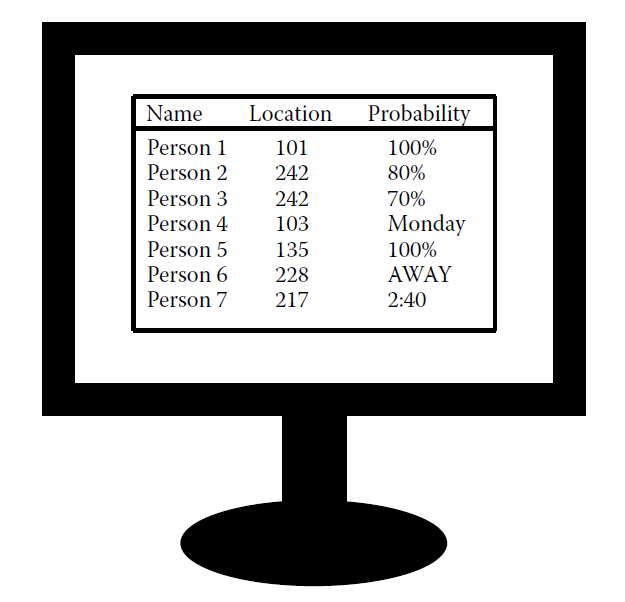
\includegraphics[scale=0.4]{images/active_badge}
\caption{Приказ од оригиналната апликација „активна значка“ кон локацијата со
соодветната веројатност на носителите на „Активна Значка“}
\label{fig:active_badge}
\end{figure}

\section{Апликации со знаење за контекстот}

Во овој дел ќе бидат опишани некои историски значајни апликации со знаење за
контекстот со кои започнува оваа област, како и некои по современи примери на
апликации во кои може да се препознае користење на контекстот.

Една од првите апликации која се смета дека прва активно го разгледува и користи
контекстот на корисникот е системот Активна значка (Active Badge) [15]. Во оваа
апликација (Слика 1) корисниците носат Активни значки, со инфрацрвени
трансмитери кои испраќаат уникатен идентификациски код. Како што корисниците се
движат низ нивната зграда, базата на податоци се менува динамички со
информацијата за локацијата на секој од корисниците, најблискиот пристап до
телефон, како и веројатноста дека ќе најдете некој на таа локација (врз основа
на староста на податоците). Кога ќе се добие повик за одреден корисник,
рецепционерот ја користи базата на податоци да го пренасочи повикот кон
последната локација на која е забележан корисникот, наместо само слепо да го
пренасочи повикот кон канцеларијата на корисникот во која тој можеби и не се
наоѓа. Оваа апликација, заедно со многу други од првичната работа во полето на
пресметувањето со знаење за контекстот се фокусирани на пресметување со знаење
на локацијата на корисникот. Ваквите апликации денес се познати и како
локациски-базирани апликации или сервиси.

Втората почетна работа во оваа област е изработена од Ubicomp group во Xerox
Palo Alto Research Center (PARC) во раните 1990ти. Во нивната работа [12] го
воведуваат терминот знаење за контекстот и развиваат архитектура на систем за
поддршка и развој на апликации со знаење за контекстот како дел од нивната
влијателна работа PARCTAB [16]. Во овој систем информациите им се презентираат
на корисниците во зависност од нивната близина до сервисите (на пример, печатачи
и луѓе), уредите се вклучуваат или конфигурираат врз основа на луѓето кои се
наоѓаат во близина, се презентираат информации или сервиси врз основа на
локацијата на корисникот и автоматски се извршуваат сервиси на начин кој зависи
од движењето или близината на корисниците до одредени соби или уреди.

Од тогаш наваму, постојат многу примери на апликации во кои е применето знаењето
за контекстот и истите се имплементирани во огромен број на домени. Сепак во
пракса се издвојуваат три главни класи на апликациски домени и тоа: туристички
водичи, системи за потсетување и контрола на околината.

\subsection{Мобилни туристички водичи}

Мобилниот туристички водич е најчестиот и нај типичен пример на апликација со
знаење за контекстот. При интеракцијата на корисникот со еден ваков систем кога
тој посетува некој музеј или град тој со себе носи преносен компјутерски уред.
Како што корисникот се движи на различни локации, неговиот мобилен уред
прикажува информации релевантни за тие локации. Иако првичните системи прилично
се базираат на локацијата [17][18], некои подоцнежни системи ги земаат предвид и
интересите на корисникот како и времето кое корисникот сака да го помине на
одредена туристичка локација или колку време може да потроши корисникот за
одредена туристичка тура [6][19].

\subsection{Потсетници} 

Вториот пример на типични апликации со знаење за контекстот се системи
потсетници. Потсетниците со знаење за контекстот презентираат потсетници на
корисникот, поттикнати од некои измени во контекстот. Алармниот часовник е една
од нај познатите вакви апликации и функционира со користење на едноставен
контекстуален активатор, време, да вклучи аларм, едноставна форма на потсетник.
Слично, локациски-базирани сервиси може да поттикнат некои потсетници кога
корисниците се на одредена локација или се на некое растојание еден од друг [4].
По софистицирани потсетници користат комбинација од различни форми на контекст
да вклучат некои потсетник. Со тоа што се по софистицирани, овие апликации може
да ги потсетуваат корисниците на по соодветен начин, со што го вклучуваат
вистинскиот потсетник во вистинската ситуација [14][20].

\subsection{Контрола на околината} 

Третиот вид на апликации со знаење за контекстот е систем за контрола на
греењето, осветлувањето или други својства на околината, со цел да се подобри
ефикасноста и да се постигне одредена заштеда на енергија. Како што луѓето сè
повеќе без потреба ги оставаат вклучени светлата, или треба рачно да го менуваат
нивото на затоплување или ладење за да се чувствуваат удобно, развиени се многу
системи кои во овие случаи ја преземаат контролата од корисникот. Некои се
засновани на прилично едноставни правила [21], додека некои други користат многу
пософистицирани методи како некои техники на машинско учење за да научат како
корисниците го користат просторот и соодветно ги постават нивото на затоплување
и осветлување [22].

\subsection{Современи апликации со знаење за контекстот}

Иако овие апликации од денешен аспект можеби изгледаат доста едноставно, сепак
вакви апликации се уште се развиваат од страна на истражувачите, а што е уште
позначајно многу од овие апликации почнуваат да излегуваат од светот на
истражувањето и да се претвораат во комерцијални апликации кои се широко
распространети. Покрај трите основни домени, истражувачите и развивачите
развиваат апликации во многу различни домени вклучувајќи ги следните:

\begin{itemize}
  \item Меѓусебна комуникација со кратки пораки [23]
  \item Вознемирување додека сме во канцеларија или додека сме мобилни [24]
  \item Телефонски повици [25]
  \item Здравствена заштита [26]
  \item Локациски-базирани системи
  \item Персонализација на апликации [27]
  \item Периферни прикази на информации [28]
\end{itemize}  

Ова е една огромна листа и наместо да се надополнува или пак да се зборува за
деталите на овие апликации, при што сето ова може да биде веќе застарено многу
скоро, многу е важно да се напомене дека истражувањето во ова поле е во добра
насока. Со самото тоа што се движи од апликации за помалку корисни работи и игри
со мал придонес за реални корисници во реални ситуации кон по фундаментални
проблеми кои се однесуваат на сите аспекти од секојдневниот живот и критични
ситуации. Ова поле ја помина фазата на зреење и сега истражувачите и развивачите
го посветуваат нивното внимание не само прикажувајќи што може да се направи и
што сè е можно, туку на она што е по убедливо и заслужува поголемо внимание.

Уште еден значаен момент е и забелешката дека голем број на истражувачи работат
на развој на апликации со знаење за контекстот, но нивниот фокус не е
контекстот. Тие едноставно развиваат корисни, значајни апликации кои едноставно
случајно го користат и контекстот. Иако ова може да се смета и како мала
дискриминација, сепак знаењето за контекстот ќе достигне ниво на зрелост кога
често на него ќе се гледа како на една од можностите на апликацијата, а не
нејзин основен фокус.

Еден од поинтересните примери за современа мобилна апликација со знаење за
контекстот е мобилна апликација која служи како личен тренер во извршувањето на
секојдневни физички активности. SportyPal [29] е токму ваков вид на мобилна
апликација во која контекстот на корисникот е всушност основната идеја во целата
апликација. Во оваа апликација корисниците избираат некоја спортска активност
како трчање, одење, планинарење или возење велосипед, по што апликацијата
постојано го следи и снима нивното движење. Исто така им пресметува моментална
брзина на движење, поминато растојание и потрошени калории. Во овој вид на
апликации контекстот го претставува локацијата на корисникот како и нејзиното
менување преку постојаното движење на корисникот. Ова е пример на апликација во
која единствено преку следење и запишување на информациите за контекстот на
корисникот може да се имплементира современа и корисна мобилна апликација. Втор
интересен пример на современа мобилна апликација со знаење за контекстот е
апликацијата Locale [30] во која во зависност од контекстот на корисникот
автоматски се нагодуваат прилагодувањата на мобилниот телефон. Се врши
прилагодување на начинот на ѕвонење, осветленоста на екранот, безжичните мрежи и
други нагодувања кои се директно засегнати од елементите на контекстот на
корисникот како локацијата, времето од денот, амбиентот во просторијата и други.

\section{Дизајн и имплементација на апликации со знаење за контекстот}

Во овој дел е опишан начинот и алатките кои постојат за дизајн и имплементација
на апликации со знаење за контекстот.

\subsection{Процес на дизајн}

Процесот на дизајн на повеќето од апликациите со знаење за контекстот може да се
сведе на прилично едноставна идеја: откривање и одредување на видот на
контекстот кој и е потребен на вашата апликација, кога го примате тој контекст и
што сакате да правите со него. Сепак, потребно е уште малку повеќе работа за да
се развие апликација со знаење за контекстот претставена преку чекорите на
Табела 1. Првиот чекор во развојот е спецификацијата на контекстот - одредување
на кои елементи од контекстот ќе се обработуваат во апликацијата и што ќе се
извршува во самата апликација врз основа на овие контекстуални информации.

Табела 1. Чекори во развојот на апликацијата за споделување на активноста во
оддалечена просторија 

Чекор   Пример Спецификација Вклучување различно обоени ЛЕД диоди (црвена, жолта, зелена) во зависност од
нивото на активност во оддалечената локација Преземање   Пишување софтвер за
анализирање на промените на сликите (frame-by-frame) од видео камера од
оддалечена локација и инсталација на камерата Прием   Објавување на информации
како нивото на активност кои може да се искористат во други апликации со
користење на пристапот со објавување/пријавување Испорака    Апликацијата сака
да ги прими сите промени на активноста над одредено ниво Акција  Апликацијата ги
анализира примените промени на активноста и ги вклучува соодветните ЛЕД диоди
(црвена, слаба активност; жолта, средна активност; зелена, висока активност)

Овој чекор вообичаено се прави преку проучување на доменот на апликацијата,
нејзините корисници и одредување кои сервиси би било корисно да им се понудат.
Вториот чекор е преземање на контекстот - одредување кој вид на хардвер и
софтвер се потребни да се собере контекстот одбран во првиот чекор. Ова вклучува
инсталација на софтверот на соодветната платформа, детално запознавање со
видовите информации кои ги овозможува сензорот, искористување на апликациски
интерфејс за програмирање (API) (ако постои) за комуникација со сензорот,
одредување на начинот на кој ќе се чита сензорот и како ќе известуваме за сите
промени на сензорот. Исто така, доколку е возможно, податоците од контекстот се
запишуваат и се комбинираат со други податоци, а се применува и учење и
одлучување за да се дојде до знаење за ситуацијата на повисоко ниво. Третиот
чекор е испорака на контекстот - спецификација како ќе се пренесе контекстот од
сензорите (кои може да се на оддалечена локација) до апликациите кои ќе го
користат контекстот. Четвртиот чекор е прием на контекстот - во кој апликациите
специфицираат кој контекст им е потребен (можно е и спецификација од кои
сензори) и примање на соодветниот контекст. Ова вклучува претворање на
контекстот во форма која е корисна од страна на апликацијата преку негова
интерпретација, а потоа и соодветна анализа дали овој контекст во комбинација со
други информации, опишува релевантна ситуација за корисникот и за апликацијата.
Последниот чекор е акцијата - анализирање на севкупниот контекст кој е примен и
одредување која акација треба да се изврши и извршување на таа акција. Иако
апликациите може да се многу по сложени од ова, сепак повеќето апликации се
опишуваат преку овој едноставен процес на дизајн.

\subsection{Алатки за развој}  

Врз основа на предложениот процес на дизајн, развиени се неколку алатки или
софтверски архитектури за поддршка на развојот на апликации со знаење за
контекстот. Ако за првиот чекор на спецификација може да се каже дека е
задолжителен во развојот на сите апликации, останатите чекори може да се
избегнат во зависност од тоа што овозможува алатката која се користи за развој.
Во најдобар случај, спецификацијата на ситуациите од интерес и соодветните
контекстно базирани однесувања се доволни за контекстот да се пренесува од
соодветните сензори до апликациите, со соодветно резонирање и интерпретација, а
потоа и соодветно извршување на акција.

\begin{figure}[htb]
\centering
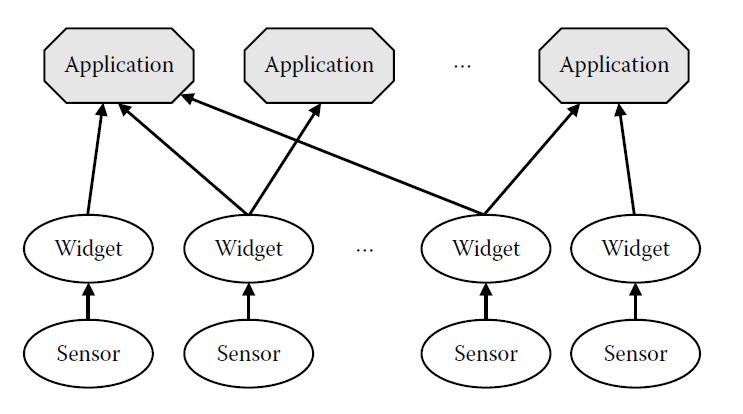
\includegraphics[scale=0.4]{images/widget_based}
\caption{Систем за развој на апликации со знаење за контекстот заснован на
објекти (widgets)}
\label{fig:widget_based}
\end{figure}
 
Постојат три основни алтернативи кои се користат за развој на апликациите: без
поддршка, систем заснован на објекти (Widgets) прикажан на Слика 2 и систем
заснован на школска табла (Blackboard). Поголемиот дел од системите, посебно тие
развиени пред 1998, се развиени без соодветна архитектура или со голема
прилагодливост кон мало множество на апликации. За секоја од овие апликации,
целосниот процес на дизајн мора да се примени поединечно за секоја од нив. Многу
малку, ако и воопшто некаков изворен код може повторно да се искористи меѓу
различни апликации, така што поголем дел од изворниот код е прилагоден за секоја
од апликациите соодветно.

Основниот пристап со објекти се
заснова на моделот на развој на графичките кориснички интерфејси (GUIs). Во
раните 1980ти, не постоел генерален модел за справување со корисничките податоци
и не постоела можност за повторно искористување на објекти кои би се справувале
со тоа. Во средина на 1980тите, се појавуваат првите GUI алатки кои поддржуваат
повторно искористување, притоа вклучувајќи ја во себе севкупната инфраструктура
за справување со настаните при внесување податоци и библиотека на компоненти што
може да се користат во повеќе различни апликации. Овие алатки го олеснуваат
развојот на графичките кориснички интерфејси со овозможување на следните
придобивки:

\begin{itemize}
  \item Тие ги сокриваат спецификите на уредите за физичка интеракција
од програмерот на апликацијата со што овие уреди може да се менуваат и притоа
настанатите промени да немаат големо влијание на апликациите. Дали корисникот
покажува или клика со глувче или покажува и допира со прсти или користи
скратеници од тастатура не предизвикува никакви измени во апликацијата.
\item Се справуваат со деталите на интеракција за да и овозможат на апликацијата
релевантни резултати од акциите на корисникот. Апликациите едноставно треба да
имплементираат некоја функција во која се враќа резултатот од интеракцијата на
корисникот.
\item Овозможуваат градбени блокови за презентација кои може да се
искористуваат и комбинираат во повеќе апликации. Тие претставуваат апстракција
на изгледот и однесувањето, а програмерот не треба да знае како се изградени за
да ги користи.
\end{itemize}

На сличен начин, во доцните 1990ти и раните 2000ти, се појавуваат софтверски
алатки за управување со контекстот како што се Context Toolkit [31] и Java
Context-Aware Framework [32] кои на сличен начин го прилагодуваат овој модел на
објекти енкапсулатори на однесување и акции. Контекст виџет е софтверска
компонента која овозможува апликациите да пристапат до контекстни информации од
нивната извршна околина. На ист начин како што GUI виџетите ги изолираат
апликациите од презентациски работи, така контекст виџетите ги изолираат
апликациите од работи како преземање на контекстот преку обезбедување на
стандарден интерфејс кон сензорите. Контекст виџетите ги овозможуваат следните
предности:

\begin{itemize}
  \item Овозможуваат издвојување на засебните и концептуално
различни делови со што ја сокриваат комплексноста на сензорите кои се користат
во апликацијата. Дали присуството на луѓето се забележува со користење на
активни значки, сензори на подот, обработка на слики или комбинација од нив нема
влијание во дизајнот на апликацијата.
\item Тие ги апстрахираат контекстуалните
информации да одговараат на барањата на апликациите. Виџет кој ја следи
локацијата на корисникот во некоја зграда или град ја известува апликацијата
само кога корисникот се движи од една соба во друга или кога од една улица
преминува на друга, а не известува за помалку значајни движења. Со неколку
зборови овозможуваат апстрахирани информации кои очекуваме дека се најпотребни
во самата апликација.
\item Овозможуваат едноставен пристап до контекстни податоци
преку механизам на пребарување и нотификација (на пример објави/пријави)
овозможен преку стандарден интерфејс за пристап на контекстот. Без разлика каков
контекст се собира од околината, сите виџети го овозможуваат на ист начин.
\item Овозможуваат градбени блокови за восприемање на контекстот кој се прилагодливи и
може повторно да се искористуваат. Виџет кој ја следи локацијата на корисникот
може да се користи во многу различни апликации, од туристички водичи се до
системи за следење на канцелариски простории. Понатаму, овие виџети може да се
комбинираат слично како и GUI виџетите. На пример, нека постои виџет кој
забележува присуство на луѓе во просторија. Над овој виџет може да се развие нов
виџет кој ќе забележува состанок кога ќе се забележи присуство на повеќе од еден
човек во просторијата. 
\end{itemize}

Како додаток на контекст виџетите, оваа инфраструктура овозможува компоненти за
комбинирање на контекстни информации, извлекување на заклучоци на повисоко ниво
од контекстот на пониско ниво, собирање и групирање на контекст од различни
извори и откривање на соодветни компоненти. Како колекција, виџетите не само што
овозможуваат компоненти кои може да се искористат за развој на поединечни
апликации, туку служат и како дистрибуирана инфраструктура која може да
поддржува повеќе апликации истовремено. Ова е пристап кој е се повеќе застапен
во реални софтверски пакети, а и доста популаризиран со самото вклучување на
апликациски интерфејс за програмирање (API) за сензорската и локациската
платформа во Microsoft Windows 7 кој овозможува пристап до сензори за локација и
осветленост и овозможува развој на апликации со знаење за контекстот.

\begin{figure}[htb]
\centering
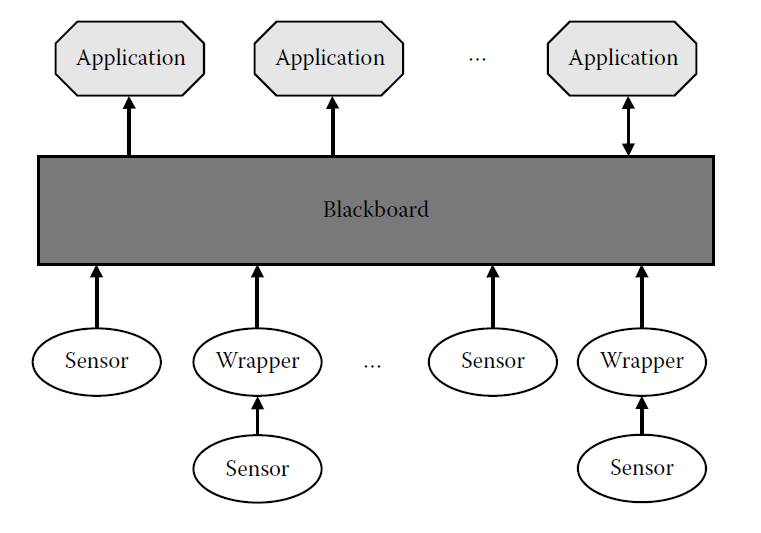
\includegraphics[scale=0.4]{images/blackboard}
\caption{Систем за развој на апликации со знаење за контекстот заснован на
школска табла (Blackboard)}
\label{fig:blackboard}
\end{figure}
 
Другиот спротивен пристап на пристапот со виџети е моделот на школска табла.
Темните табли (blackboards) имаат зачетоци од програмскиот јазик Linda и моделот
на простор на листи од парови во раните 1980ти [33]. Програмскиот јазик Linda
овозможува мал број функции за интеракција со глобален систем за перзистирање,
наречен простор на листа од парови (tuple space). Извршни компоненти може да
запишуваат, читаат или бришат информации во овој систем. Подоцна системите со
школска табла ја додаваат можноста да ги известуваат компонентите кога
информациите од интерес се додадени во таблата. Наспроти пристапот со виџети кај
кои барањата за информации се вршат директно врз компонентите преку механизам за
откривање, пристапот на школска табла овозможува барања за информации да доаѓаат
и се справуваат од единствен, централизиран простор на листи од парови. Воопшто,
контекст системите засновани на школска табла се едноставна имплементација на
традиционалните системи со темни табла, оптимизирани за перформанси и збогатени
со поддршка за XML енкодирање и декодирање на информациите.

И двата пристапи имаат свои предности и недостатоци. Пристапот на школска табла
е многу често неефикасен, особено кога количеството на податоци расте и
просторот на листи со парови се зголемува со што пребарувањето на одредени
парови станува многу тешко. Исто така, многу често овој систем е премногу силно
интегриран со апликацијата што предизвикува проблеми со синхронизацијата. Овој
проблем предизвикува задоцнување во модификација на апликацијата, конкретно во
просторот со податоци кој е ограничен поради тоа што не подржува комплексни
податочни структури. Моделот заснован на виџети исто така има доста проблеми од
аспект на робустност и конфигурација, со што тешко се справува со динамичката
природа на апликациите со знаење за контекстот, затоа што овие апликации имаат
потреба да се поврзуваат и исклучуваат од одредени компоненти како што
корисникот се движи, а неговиот контекст се менува.

Меѓутоа, овие два пристапи и не се меѓусебно исклучиви. Од перспектива на
развивач на инфраструктура, и за двата пристапи се потребни извори на контекст,
дали да се креираат виџетите или да се внесе контекстот во просторот со листи од
парови. Пристапот со контекст виџети овозможува добар модел за ефикасно
искористување на изворите на контекст, без разлика кој пристап се користи во
самата апликација. Од друга страна, моделот со школска табла овозможува
поедноставна апстракција на овие извори на контекст и го поедноставува
пренесувањето на контекстот до неговите консументи. Овој модел може да се
искористи во пристапот со виџети, каде на виџетите може да им се наложи да се
поврзат на некоја централизирана компонента (на пример, систем за откривање),
кој ќе одреди кој и каков ќе биде патот на контекстот од виџетот до консументот.
Од перспектива на развивач на апликации работата е многу олеснета со можноста да
се сокријат деталите на технологијата на сензорите и вчитувањето на контекстот
преку виџети. Нема потреба да се грижиме за индивидуалното поврзување на
компонентите во апликацијата со контекстот преку темни табли или контекст виџети
и механизмот за откривање.

\section{Проблеми во развојот на апликации со знаење за контекстот} 

Во овој дел се разработени аспектите на кои треба да им се посвети особено
внимание во развојот на апликациите со знаење за контекстот. 

\subsection{Контекстот како прокси за човечката намера}

Крајната цел на знаењето за контекстот е преку него да се дознае намерата на
корисникот. Апликациите ќе ја искористат оваа намера на човекот за соодветно да
се прилагодат преку обезбедување информации или преземање некакви акции.
Меѓутоа, информациите за контекстот се само прокси за оваа намера. Во
туристичките водичи во музеј, кога корисникот стои до одредена изложба може да
претставува дека корисникот има интерес кон неа, но може и да значи дека тој е
свртен со грб кон изложбата и разговара со пријател. Ваков е случајот во скоро
сите ситуации и апликации. Без разлика колку контекст може да се обработи во
апликацијата, секогаш е потребно повеќе за да се одреди вистинската намера на
корисникот. Кога се дизајнира апликација, развивачите мора да го дефинираат
опсегот на видови на ситуации кои апликацијата ќе ги препознава и разбира и
притоа помирувајќи се со фактот дека апликацијата може да направи неточно
прилагодување кон одредена ситуација кога таа ситуација е надвор од опсегот на
дизајнираната апликација. Апликацијата треба да искажува и некаква
веродостојност на нејзиното верување за одредена ситуација која е препознаена,
како што тоа го прави на пример системот со Активни Значки (слика 1). Ако
веродостојноста не е над некоја одредена граница, може да се побара и потврда од
корисникот пред да се изврши некоја акција, што е применето на пример во агентот
Clippy на Microsoft и во Lookout system [34].

\subsection{Препознавање на контекстот и проблеми во препознавањето}  

Системите со знаење за контекстот примаат некакви податоци на влез и одредуваат
и одлучуваат како ќе одговорат на овие податоци. Препознавање на контекстот е
делот во кој од податоците од сензорите треба да се добие разумен заклучок за
ситуацијата во која се наоѓа корисникот. Откако ќе се препознае ситуацијата на
корисникот, апликацијата може да преземе соодветна акција. Како што веќе е
споменато, скоро секогаш влезните податоци се недоволни да се препознае
соодветната ситуација, така да ова носи дополнителни проблеми од тоа како да се
разреши оваа несигурност во контекстот и улогата на правилата и машинското
учење.

Системите со знаење за контекстот имаат многу извори на недоследност, грешки или
тешкотии во препознавањето: сензорите како извори на контекстот може да работат
неточно, да откажат или да бидат несигурни во своите податоци; системите за
препознавање на контекстот може да бидат непрецизни или да носат неточни
заклучоци за одредена ситуација или бидат несигурни во своите заклучоци и
апликациите може да извршат неточни акции или да бидат несигурни која акција
треба да ја извршат. Повеќето системи со знаење за контекстот го сокриваат ова
или едноставно се однесуваат како да не постои. Една од важните одлуки за
дизајнерите која треба да ја донесат е дали да го моделираат контекстот со
можност за непрецизност или не. Однесување како да не постојат грешки и
непрецизности го поедноставува целиот процес на дизајн, но води кон не
флексибилни системи во однос на прецизноста на податоците. Спротивно, прифаќање
дека грешките и недостатоците постојат значи дека се моделираат системи кои
подобро го отсликуваат реалниот свет, но внесуваат и повеќе предизвици во
развојот и користењето. Грешката често се специфицира со некаков број кој
претставува веројатност или веродостојност на одредена вредност од контекстот.

Еден од пристапите за справување со непрецизноста на контекстот е да се
комбинираат повеќе различни извори за истиот вид контекст со цел да се подобри
прецизноста. Ова е познато како спојување (фузија) на сензори [35]. На пример,
при препознавање на активност, може да се искористи скриен Марков модел со
различни сензори и споените резултати да се репрезентираат како резултатна
матрица (confusion matrix) на множеството од можни активности [36]. Алтернативен
пристап е да им се овозможи на корисниците самите да ја разрешат несигурноста во
контекстот [37]. Наместо да се потпира целосно на автоматизиран процес, овој
пристап го користи знаењето на корисникот за ситуацијата да помогне во
разрешувањето на несигурноста во вчитаниот и одреден контекст. На корисникот
може да му се понуди листа од на пример N најдобри интерпретации на контекстот
со најголема веројатност и точност, а потоа да се побара да ја избере „точната“
интерпретација.

\subsection{Правила наспроти машинско учење}  

Апликациите со знаење за контекстот најчесто се дизајнираат со множество на
ако/тогаш правила: ако апликацијата препознае некоја одредена ситуација, тогаш
треба да изврши одредена акција. Правилата се создаваат едноставно, затоа што
целото знаење за секое од правилата е хомогено репрезентирано и овие системите
засновани на правила релативно лесно се развиваат затоа што постојат голем број
на постоечки под-системи кои одредуваат кога некое правило е задоволено.
Правилата се исто така доста интуитивни и едноставни за работа. Меѓутоа, овие
системи имаат и свои недостатоци: тие се склони кон создавање конфликти меѓу
правилата поради некоја скриена зависност, со што е прилично тешко кога треба да
се додаде некое ново правило, посебно кога бројот на правила е доста голем.
Едноставно тешко е да се следи текот на контролата меѓу правилата, а тие се исто
така и извор на не ефикасност, затоа што системот за одлучување преку правила
мора да ги измине сите правила за да одреди дали некое правило, ако воопшто, е
задоволено. Мали исклучоци кон некое правило може да значат дека тоа правило не
е исполнето или некое сосема друго правило е исполнето (она кое го претпочита
развивачот).

Познат алтернативен пристап е да се примени машинско учење. Наместо да се
создава листа на правила за тоа како апликацијата треба да се однесува,
развивачот на апликацијата може да собира податоци од видовите на ситуации со
кои се соочуваат корисниците и видовите на акции кои ги посакува. Потоа може да
се примени машинско учење да се научи веројатносната врска меѓу ситуациите и
акциите, наместо овие врски да се кодираат и бидат детерминистички. Ова сè уште
бара од апликацијата да овозможи инфраструктура и можности за прибирање на
контекстот и иницијално преведување на сензорските податоци во соодветната
ситуација. Машинско учење може да се примени и во врската меѓу сензорските
податоци и акциите, со што ќе се прескокне средниот чекор на идентификација на
контекстот. Недостатоците на овој пристап се што може да биде тешко да се научат
врските, а можно е и да е потребно големо количество податоци. Исто така ова се
прилично тешки методи за детектирање и отстранување грешки, а и не се интуитивни
за развивачот на апликацијата или крајниот корисник.

\subsection{Приватност}    

Системите со знаење за контекстот често имаат потреба да собираат големи
количества на лични информации за индивидуалците. Она што секогаш постои како
опасност при собирањето на вакви приватни податоци е можноста да се објават на
погрешни луѓе или во погрешни ситуации. Конкретно, затоа што овие системи
најчесто се дистрибуирани на повеќе компоненти и компјутерски мрежи, постои
реална можност да овие контекстни информации се дисиминираат несоодветно или пак
да се дисеминраат на компонента на која не може да и се верува. При развојот,
развивачите треба да обезбедат овие приватни информации да се споделуваат само
меѓу компонентите кои вистински имаат потреба да ги користат и споделуваат овие
информации. Исто така, развивачите треба да обезбедат да се зачувува приватноста
на корисникот и информациите да не се користат на несоодветен начин или на начин
за кој корисникот смета дека е несоодветен. Проблемот на приватноста е доста
комплексен и вообичаено се разработува посебно. Не постојат едноставни одговори
за тоа како да се обезбеди задоволителна приватност.

\subsection{Евалуација}    

Апликациите со знаење за контекстот, покрај многуте специфичности се одликуваат
и со својството дека се тешки за евалуација. Затоа што овие апликации се зависни
од контекстот, ретко може да се тестираат во лабораториска околина. Многу е
тешко да се симулира контекстот или ситуацијата од интерес. Дури и при
евалуација на терен, некои од овие ситуации се многу ретки така што голем е
предизвикот да се тестира и евалуира на различен аспект од квалитативен. Како да
се евалуираат овие апликации е исто така интересна тема за истражување и тема на
некои тековни истражувања [38][39][40].
